% 2006 天津理科 Q22；固定候选 PDF 第 2 页（印刷页 337）。
% 几何示意按 a=1, b=(sqrt(5)-1)/2 归一化，满足 c^2=ab 与 c>b；不表示题目比例要求。
% 大圆/小圆半径分别为 a,b；椭圆为 x^2/a^2+y^2/b^2=1。A 在 x=c 竖线上，
% B 在 OA 上且属于小圆，BF 为小圆在 B 点的切线，并交椭圆于 P,Q。
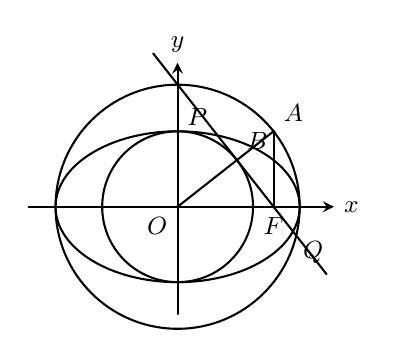
\begin{tikzpicture}[x=1.55cm,y=1.55cm,line cap=round,line join=round,line width=0.75pt,font=\small,>=stealth]
  % 归一化参数：a=1, b=(sqrt(5)-1)/2, c=sqrt(a b)
  \def\bb{0.618}
  \def\cc{0.786}
  \def\yy{0.618}
  \coordinate (O) at (0,0);
  \coordinate (F) at (\cc,0);
  \coordinate (A) at (\cc,\yy);
  \coordinate (B) at (0.486,0.382);
  % 椭圆、同心圆与坐标轴
  \draw (0,0) ellipse [x radius=1,y radius=\bb];
  \draw (O) circle [radius=1];
  \draw (O) circle [radius=\bb];
  \draw[->] (-1.22,0)--(1.28,0) node[right] {$x$};
  \draw[->] (0,-0.88)--(0,1.18) node[above] {$y$};
  % OA、垂线 x=c、切线 BF；P,Q 为切线与椭圆的实际交点
  \draw (O)--(A);
  \draw (\cc,0)--(A);
  \draw (-0.20,1.256)--(1.22,-0.552);
  % 关键点标记
  \fill (O) circle (0.7pt);
  \fill (A) circle (0.7pt);
  \fill (B) circle (0.7pt);
  \fill (F) circle (0.7pt);
  \node[below left] at (O) {$O$};
  \node[above right] at (A) {$A$};
  \node[above right] at (B) {$B$};
  \node[below] at (F) {$F$};
  \node[above left] at (0.327,0.584) {$P$};
  \node[below right] at (0.945,-0.202) {$Q$};
\end{tikzpicture}
